% !TEX program = pdflatexmk

% The line above is a directive for TeXShop and TeXworks.
% - For TeXShop: this directive enables one-click typesetting for this file, 
% 	instead of the multi-step process usually needed for BibTeX.
% - For TeXworks: the directive will only work after TeXworks has been 
% 	configured to use latexmk; see 
% <https://github.com/TeXworks/texworks/wiki/AdvancedTypesettingTools> 

\documentclass[11pt]{amsart}

\usepackage[letterpaper,left=125pt,right=125pt]{geometry}

% ^^^^^^^^^^^^^^^^^^^^^^^^^^^^^^^^^^^^^^^^^^^^^^^^^^^^^^^^^^^^^^^^^
% DO NOT change anything above this line! 
% (We need standard margins and type size.)
% In particular, don't include your own "geometry" settings further down.



%%%%%%%%%%%%%%%%%%%%%%%%%%%%%%%%%%%%%%%%%%%%%
% The following part of the preamble sets up packages, theorems, and shortcuts; 
% you can edit it, but you won't need to change much.

%% Load Packages:

\usepackage[english]{babel}
\usepackage {amsmath}  % provides lots--- e.g. equations, matrices, definition by cases
\usepackage{amssymb}  % provides common mathematical symbols
\usepackage{amsfonts}
\usepackage{amsthm}     %provides \newtheorem, \theoremstyle, \begin{proof}...\end{proof}
\usepackage{graphicx}  % allows importation of graphics files
\graphicspath{{./}{Figures/}{Figures/Feature Importance/}{Figures/ROC Curves/}{Figures/Confusion Matrices/}}
\usepackage{adjustbox}
\usepackage{booktabs}
\usepackage{float}
\usepackage{placeins}
\usepackage[colorlinks,linkcolor=blue,citecolor=blue,urlcolor=blue]{hyperref} % typesets URLs and clickable cross-references and links
%\usepackage{hyperref} % if you don't want colored links, just use the simpler command
\usepackage{listings}
\usepackage{xcolor}


\lstset{
    language=Python,
    basicstyle=\ttfamily\small,
    keywordstyle=\color{blue},
    stringstyle=\color{red},
    commentstyle=\color{green!50!black},
    showstringspaces=false,
    breaklines=true,
    frame=single
}

%% Bibliography support
\usepackage[backend=biber,sorting=nty,isbn=false,url=false]{biblatex} 
% notes on settings:
% backend=biber: we are using the newer tool biber for processing (rather than the older bibtex program)
% isbn=false, because printing ISBNs is distracting clutter
% urls=false: we don't need to show URLs for primarily print sources (distracting); 
%							this setting does *not* apply to `@online` records 

\addbibresource{bib.bib}


%% Environments for theorems, etc.. 

% You can add your own theorem-like environments, see https://en.wikibooks.org/wiki/LaTeX/Theorems
% The basic formats are 
% \newtheorem{name}{display-text}[numbered-within]  and
% \newtheorem{name}[numbered-like]{display-text}

\newtheorem{thm}{Theorem}[section] %\newtheorem{name}{display-text}[numbered-within]

\newtheorem{lem}[thm]{Lemma} %\newtheorem{name}[numbered-like]{display-text}
\newtheorem{cor}[thm]{Corollary}
\newtheorem{prop}[thm]{Proposition}
\newtheorem{alg}[thm]{Algorithm}

% the batch of theorem-like environments above are typeset in the default "plain" style, with italic text

\theoremstyle{definition}                  % switch to a different style: roman text and extra spacing above and below
\newtheorem{defn}[thm]{Definition}
\newtheorem{conj}[thm]{Conjecture}
\newtheorem{prob}[thm]{Problem}

\theoremstyle{remark}                       % switch to yet another style: roman text, no extra spacing
\newtheorem{exmp}[thm]{Example}  
\newtheorem{rem}[thm]{Remark}
\newtheorem{claim}[thm]{Claim}  

%% If you use numbered equations in a long document, it is preferred to number
% as (x.y), where x is section number, y is equation number

\numberwithin{equation}{section}


%% Common typesetting for common mathematical objects

\newcommand{\R}{\mathbb{R}}
\newcommand{\Q}{\mathbb{Q}}
\newcommand{\N}{\mathbb{N}}
\newcommand{\Z}{\mathbb{Z}}
\DeclareMathOperator{\rank}{rank}
\DeclareMathOperator{\dimension}{dim}



%%%%%%%%%%%%%%%%%%%%%%%%%%%%%%%%%%%%%%
% BEGIN: You'll _need_ to edit everything below....


%  Your data for title, author, etc.

\title[A Closer Look at One-Score Games In College Football]{A Closer Look at One-Score Games In College Football} % here, the command format is  \title[Abbreviated Title for Header]{Full Title}. But if your title is short, simply use \title{Full Title}
\thanks{This document is a senior thesis submitted to the Department of Mathematics and Statistics at Haverford College in partial fulfillment of the requirements for a major in Mathematics.} % REQUIRED: don't change this line
\author{Haroun Shah}
\date{March 6, 2026} % don't forget to update the date!

\begin{document}

\begin{abstract} % REQUIRED (and needs to go before \maketitle)
In this senior thesis, we will enter the world of sports analytics by utilizing machine learning to investigate ``one-score games" in college football, that is, games ending with a point differential of 8 points or less. These close matchups are often hard to predict due to the many variables that could drastically sway the outcome. We identify the in-game team statistics that are most indicative of success in winning these games. Our findings could prove to be applicable for players, coaches, and managers aiming to improve their university's football program. It is important to keep in mind that the models constructed in this senior thesis are only consistent with one-score games, and thus cannot be used to predict future matchups where point differential is not predetermined.
\end{abstract}

\maketitle % Actually typeset the title, author, etc.

\section*{Acknowledgments}
I would like to thank my thesis advisor and the faculty in the Department of Mathematics and Statistics at Haverford College for their guidance and support throughout this project. I am also grateful to my family and friends for their encouragement throughout the senior thesis process.


\tableofcontents % OPTIONAL. See https://en.wikibooks.org/wiki/LaTeX/Document_Structure#Table_of_contents for more information.

%%-------------------------------------------------------------------------------------------------
%% CUT START: you can delete all of the following content, through "CUT STOP" below
\section{Introduction}

Nowadays, every sports fan has strong opinions about their favorite teams or players, and very rarely are they hesitant to share their input. Fans like to think that they know the exact reason for their team’s poor performances, and they can always make an argument as to why their favorite player is better than the rest. Largely due to social media, fans' opinions often are shaped by the “hot-takes” and highlights seen online, but to gain a better understanding of what truly determines the results of the biggest sports games, we need to turn to the statistics.

As sports and technology have evolved in recent years, \textit{machine learning} has become integral to how coaches, teams, leagues, and sports analysts understand and evaluate performance \cite{rein2016bigdata, lewis2003moneyball}. With fairly accessible, high-quality datasets and new advancements in computational power, it’s now possible to investigate many complex questions about game strategy, team efficiency, and competitive outcomes across the world of sports. College football provides a rich environment for quantitative study due to its large number of features, diverse styles of play, and significant variability in team strength and performance from week to week. As a result, it has become quite an appealing domain for applying methods from statistics, data science, and machine learning \cite{hastie2009elements, james2021introduction}.

Among the many facets of college football, \textit{one-score games} (matchups decided by a point differential of 8 or less) represent an interesting scenario. These games are defined by narrow margins in which small changes in team/individual performance can alter the final result. Unlike “blowouts”, where clear differences in talent typically dictate outcomes, one-score contests often hinge on subtle details such as turnover margin, total yards, third-down conversion rates, or time of possession. Understanding what differentiates winning and losing performances in these tight scenarios is valuable not only for predictive modeling but also for gaining insight into how teams respond under such high-pressure conditions.

The purpose of this senior thesis is to investigate the statistical patterns and performance metrics that most strongly influence the outcomes of one-score college football games. By compiling a dataset of team statistics of one score matchups from NCAA Division I Football Bowl Subdivision (FBS) \footnote{FBS is the highest level of collegiate football in the NCAA} games played from 2014 to 2024, this senior thesis aims to explore which of these metrics are most indicative of success. The exploratory data analysis conducted in this thesis will examine the structure of the dataset, summarize/understand the key variables, identify meaningful relationships, and highlight which metrics are most closely associated with winning these close games. These findings will serve as the foundation for the next phase of the project, in which machine learning methods such as logistic regression, random forests, gradient boosting, support vector machines, and naive Bayes will be utilized to classify the outcomes of one-score games.

Beyond its value in predictive modeling, this work contributes to the broader field of sports analytics \cite{rein2016bigdata} by examining the specific statistical determinants of competitive balance in college football. Understanding the dynamics of close games is important for coaches seeking strategic advantages, analysts interpreting team performance, and team managers building the most well-rounded roster. The methods used in this project, ranging from feature engineering exploration to supervised learning, are generalizable and could be extended to other football leagues, most notably, the National Football League. Ultimately, this research aims to connect these rigorous quantitative methods with practical insights to understand one of the most uncertain yet strategically rich aspects of college football: the keys to winning close games.

\section{Data Collection}

The data collection portion
\footnote{Note: All code for data collection can be found in the  \href{https://github.com/HarounShah/Predicting-Results-of-One-Score-Games-in-College-Football}{GitHub repository} (see files ESPNCollection.py and DataCollection.py).} 
involved crafting a dataset of the relevant team stats from all one-score FBS matchups played from the years 2014 to 2024. Each game is labeled by a unique 9-digit ``game ID", which we simply retrieved from \href{collegefootballdata.com}{collegefootballdata.com} (CFBD).

\subsection{ESPN Web Scraping}
\href{https://www.espn.com/}{ESPN.com} serves as a great source for all major sports data, so we began the data collection phase by scraping ESPN's web pages (one page for each game). By simply changing the ESPN URL to include any specific game ID as follows:

\begin{lstlisting}
game_ids = onescore_data_df['Id']
game_ids = game_ids.reset_index(drop = True)

game_urls = []

for id in game_ids:
    game_urls.append(
        f'https://www.espn.com/college-football/matchup/_/gameId/{id}')
\end{lstlisting}
we were able to iterate through each web page and extract the necessary team stats. After compiling the data and selecting only the games with a point differential 8 or less, we faced the problem of missing data. Specifically, almost all of the defensive stats (e.g. sacks, tackles, pass deflections, etc.) were missing from a large majority of the seasons we looked at. Most likely, this missing data was, at one point, recorded and displayed on ESPN's website, but has since been removed in an attempt to minimize the costs of data storage and maintenance. It may also be useful to keep in mind that ESPN may prioritize the long-term storage of professional sports data from leagues like the NBA (National Basketball Association) or NFL (National Football League) over the data from college sports like NCAA football. Based on a foundational understanding of college football, these missing defensive statistics were far too important to be left out of the modeling phase, so another method of data collection was necessary.

\subsection{CFBD API}
The \href{collegefootballdata.com}{CFBD website} offers a free API key to directly query their database from a personal device. Using this method, we were able to again retrieve the game IDs, then use those to fetch the team statistics from all of the games. In total, this method retrieved data from 9,414 FBS games and included 43 features for each team (game ID, points, time of possession, etc.). See the Python code for the API queries below. This method still had some missing data; however, it appeared to be the most complete option to allow us to conduct data pre-processing.

\begin{lstlisting}
# Iterate through each week of the season
for week in range(1, MAX_WEEKS + 1):
    params = {
        "year": year,
        "week": week,
        "classification": "fbs"
    }

    # Ensure there are no issues with locating the week and/or year 
    resp = requests.get(BASE_URL, headers=HEADERS, params=params)
    if resp.status_code != 200:
        print(f"{year} week {week}: HTTP {resp.status_code}")
        continue

    # Ensure that statistical data is present
    data = resp.json()
    if not data:
        print(f"No data for {year} week {week}")
        continue

    # Flatten team stats
    for game in data:
        game_id = game.get("id")
        for team_entry in game.get("teams", []):
            record = {
                "year": year,
                "week": week,
                "game_id": game_id,
                "teamId": team_entry.get("teamId"),
                "team": team_entry.get("team"),
                "conference": team_entry.get("conference"),
                "homeAway": team_entry.get("homeAway"),
                "points": team_entry.get("points")
            }
            for stat_entry in team_entry.get("stats", []):
                cat = stat_entry.get("category")
                val = stat_entry.get("stat")
                record[cat] = val
            all_records.append(record)

    print(f"{year} week {week}: {len(data)} games ({len(data)*2} team rows)")
    time.sleep(SLEEP_TIME)
\end{lstlisting}

\section{Data Pre-Processing} 

To carry out data pre-processing\footnote{Note: All code for data pre-processing can be found in the \href{https://github.com/HarounShah/Predicting-Results-of-One-Score-Games-in-College-Football}{GitHub repository} (see file DataPrep.py).}, we labeled each row with the label/class as follows:
\[ \begin{cases} 
      1 & \text{if home team won} \\
      0 & \text{if home team lost}
   \end{cases}
\]
Then, in a similar fashion, created a new feature that compares the home team's points to the away team's, and if the difference is less or equal to than 8, it is labeled as a one-score game:
\[ \begin{cases} 
      1 & \text{if }||\text{ home team score} - \text{away team score}|| \leq  8\\
      0 & \text{if otherwise}
   \end{cases}
\]

Any columns that could be deemed unimportant or were missing large amounts of data were removed. For example, the \textit{puntReturns} feature (the number of times a team receives a punt) had over 800 missing data points, and the feature itself may not be important enough to warrant the significant decrease in training data. Similar features included \textit{kickReturns} (the number of times a team receives a kick) and \textit{totalPenaltiesYards} (the number of penalties a team receives along with the amount of yards they are penalized). After selecting just the one-score games, the number of rows (games) decreased from 9,414 to 3,239. Furthermore, after removing all rows with missing data, it decreased further to 2623 games. We are then left with two columns for each team statistic (eg., \textit{firstDowns\_home} and \textit{firstDowns\_away}). Using these features in machine learning models could be misleading and redundant. We are interested in exploring how these statistics contribute to a team \textit{winning} a game, which implies that the opposing team loses that same game. For example, even if the home team gets 20 first downs and the away team gets 27, then that should decrease the probability of any model to label this game as a win for the home team. In essence, the statistics are only indicative of a team's chances of winning when compared to the statistics of the opposing team. For this reason, a ``difference'' feature for each \_home and \_away pair is computed (eg. \textit{firstDowns\_diff} is defined as \textit{firstDowns\_home} - \textit{firstDowns\_away}). This produced data with 16 ``difference'' feature columns defined as follows\footnote{See Appendix~\ref{app:stat_features} for a brief explanation of each statistic.}:
\begin{itemize}
    \item possessionTime\_diff
    \item interceptions\_diff
    \item fumblesLost\_diff
    \item turnovers\_diff
    \item yardsPerRushAttempt\_diff
    \item rushingYards\_diff
    \item yardsPerPass\_diff
    \item netPassingYards\_diff
    \item totalYards\_diff
    \item firstDowns\_diff
    \item tacklesForLoss\_diff
    \item tackles\_diff
    \item sacks\_diff
    \item qbHurries\_diff
    \item passesDeflected\_diff
    \item thirdDown\%\_diff
\end{itemize}

\section{Exploratory Data Analysis}

With our dataset pre-processed we may now begin the exploratory analysis of our data\footnote{Note: All code for exploratory data analysis can be found in the  \href{https://github.com/HarounShah/Predicting-Results-of-One-Score-Games-in-College-Football}{GitHub repository} (see file EDA.py).} \cite{tukey1977exploratory, james2021introduction}. 

\subsection{Descriptive Statistics}
It is important that we get a good understanding of all of our features. Firstly, let's observe the numerical summary of each feature:

\begin{table}[H]
\centering
\small
\begin{tabular}{lrrrrrrr}
\toprule
\textbf{Feature} & \textbf{Mean} & \textbf{Std} & \textbf{Min} & \textbf{25\%} & \textbf{50\%} & \textbf{75\%} & \textbf{Max} \\
\midrule
possessionTime\_diff      & -15.3019 & 539.5982 & -1762.0 & -370.0 &  -34.0 &  354.0 & 1936.0 \\
interceptions\_diff       &  -0.0206 &   1.2278 &    -5.0 &   -1.0 &    0.0 &    1.0 &    5.0 \\
fumblesLost\_diff         &   0.0271 &   1.0812 &    -4.0 &   -1.0 &    0.0 &    1.0 &    4.0 \\
turnovers\_diff           &   0.0065 &   1.5876 &    -6.0 &   -1.0 &    0.0 &    1.0 &    5.0 \\
yardsPerRushAttempt\_diff &   0.0396 &   2.0226 &    -7.3 &   -1.3 &    0.1 &    1.4 &    9.3 \\
rushingYards\_diff        &   3.0698 & 108.4108 &  -458.0 &   -67.0 &  4.0 &   75.5 &  394.0 \\
yardsPerPass\_diff        &   0.0618 &   2.9772 &   -19.0 &   -1.7 &    0.1 &    1.8 &   36.5 \\
netPassingYards\_diff     &  -1.6805 & 115.7711 &  -425.0 &   -79.0 &    0.0 &   78.0 &  402.0 \\
totalYards\_diff          &   1.3965 &  99.2184 &  -375.0 &   -66.0 &    4.0 &   68.0 &  328.0 \\
firstDowns\_diff          &   0.1704 &   6.6146 &   -21.0 &   -4.0 &    0.0 &    4.0 &   23.0 \\
tacklesForLoss\_diff      &   0.0660 &   3.7975 &   -26.0 &   -2.0 &    0.0 &    3.0 &   25.0 \\
tackles\_diff             &  -1.1144 &  14.0380 &   -91.0 &   -9.0 &   -1.0 &    7.0 &   86.0 \\
sacks\_diff               &   0.1254 &   2.4958 &   -12.0 &   -1.0 &    0.0 &    2.0 &   18.0 \\
qbHurries\_diff           &   0.6901 &   2.8980 &   -15.0 &   -1.0 &    0.0 &    2.0 &   19.0 \\
passesDeflected\_diff     &   0.4258 &   3.3046 &   -18.0 &   -2.0 &    0.0 &    2.0 &   16.0 \\
thirdDown\%\_diff         &   0.0006 &   0.1660 &   -0.6  &   -0.1 &    0.0 &    0.1 &   0.6 \\
\bottomrule
\end{tabular}
\caption{Five-number summaries and descriptive statistics for all numerical features.}
\label{tab:five_number_summary}
\end{table}
Table \ref{tab:five_number_summary} gives an initial idea of the range and spread of each feature. Most features have varying scales of magnitude, but all have a mean equal to or close to 0. This is to be expected, as any mean away from 0 would hint at some sort of home-field advantage/disadvantage. Overall, nothing from this table seems to stand out or present any concern. Visualizing the features using histograms can help us build upon these initial observations.

\subsection{Distribution of Features}
The histograms of each feature, displayed in Figure \ref{fig:histograms}, show us that almost all of the features seem to follow a normal distribution centered around 0. We can observe that certain features, such as \textit{interceptions\_diff} and \textit{fumblesLost\_diff}, take only integer values.
\begin{figure}[H]
\centering
\includegraphics[width=\textwidth]{Histograms.png}
\caption{Distribution of difference features}
\label{fig:histograms}
\end{figure}

\subsection{Distributions by Class}
Separating the histograms by class is very effective in showing the relationships between each feature and the label. For example, in Figure \ref{fig:histogramsbyclass}, we can see that higher \textit{rushingYards\_diff} and \textit{possessionTime\_diff} are associated more often with the winning team, whereas \textit{turnovers\_diff} is associated with the losing team.
\begin{figure}[H]
\centering
\includegraphics[width=\textwidth]{HistogramsByClass.png}
\caption{Distribution of difference features separated by class}
\label{fig:histogramsbyclass}
\end{figure}

\subsection{Boxplots and Outliers}
The boxplots for each feature, shown in Figure \ref{fig:boxplots}, give us a good idea of the spread of each feature, while identifying any potential outliers in the data. We can see most of the features have many outliers, but this is due to the very high concentration of data points around the mean 0. Overall, there are no major concerns from these boxplots.
\begin{figure}[H]
\centering
\includegraphics[width=\textwidth]{Boxplots.png}
\caption{Boxplots of difference features}
\label{fig:boxplots}
\end{figure}

\subsection{Correlation Structure}
After having explored the distributions of each feature, we should observe feature correlations. The correlation matrix, shown in Figure \ref{fig:correlation}, allows us to observe the correlation between each pair of features. As expected, there is a relatively high correlation for turnovers and interceptions, as well as for turnovers and lost fumbles. Turnovers are comprised of fumbles and interceptions, and Figure \ref{fig:correlation} shows that turnovers are more highly correlated with interceptions than with fumbles. First downs are positively correlated with total yards and possession time, while tackles are inversely correlated with possession time and first downs. Rushing yards and passing yards also have a relatively strong negative correlation. None of these relationships, except maybe the last, should be considered surprising. Overall, we can use this information to consider which features to use in our models, and we pursue feature selection further in Tables \ref{tab:feature_tests_full} and \ref{tab:vif_full_eda}.
\begin{figure}[H]
\centering
\includegraphics[width=\textwidth]{CorrelationMatrix.png}
\caption{Correlation matrix of difference features}
\label{fig:correlation}
\end{figure}

\subsection{Class Balance}
The balance of class labels is an important factor to consider before training models. Large class imbalances can lead to misleading results, ineffective models, and thus, more effort to subdue these issues \cite{james2021introduction, fawcett2006introduction}. Across the 2623 one-score games in the training dataset, the home team won 1433 games ($54.63\%$), while the away team won 1190 games ($45.37\%$). Thus, the class distribution is only mildly imbalanced and does not require aggressive imbalance correction.

\begin{figure}[H]
\centering
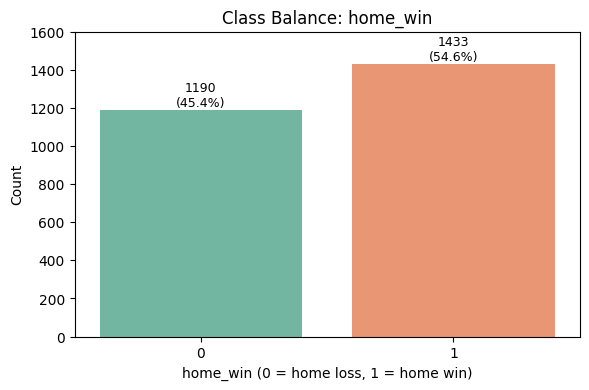
\includegraphics[width=0.65\textwidth]{ClassBalance.png}
\caption{Class balance of one-score games in the training data.}
\label{fig:class_balance}
\end{figure}
\FloatBarrier

\subsection{Win Rate by Feature Quantile Bins}
For interpretability, we can examine the home-win rate within different quantile bins of a few features of interest:

\begin{figure}[H]
\centering
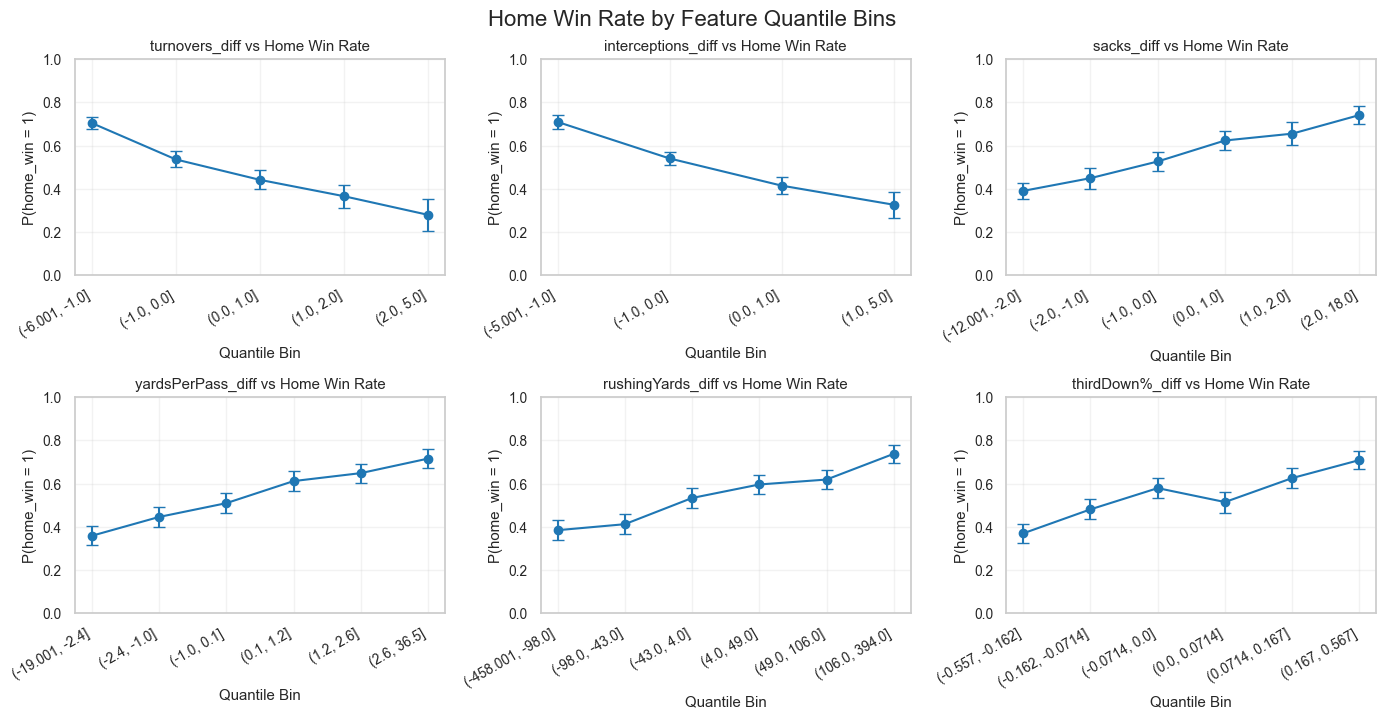
\includegraphics[width=\textwidth]{WinRateByFeatureBins.png}
\caption{Home win rate by feature quantile bins (with approximate confidence intervals).}
\label{fig:winrate_bins}
\end{figure}
\FloatBarrier

The binned win-rate trends in Figure \ref{fig:winrate_bins} reaffirm earlier correlation and test results: turnover margin features show clear monotonic trends in many bins, thus reinforcing their predictive relevance in one-score outcomes.

\subsection{Feature--Outcome Association Tests}
To complement visual inspection, each difference feature was compared between home-win and home-loss groups using Welch's two-sample $t$-test (unequal variance assumption with alpha level of 0.05) \cite{welch1947generalization} and Cohen's $d$ effect size \cite{cohen1988statistical}. This allows us to measure both statistical significance and practical magnitude of each feature's separation between classes.

Table \ref{tab:feature_tests_full} reports the full per-feature test results.

\begin{table}[H]
\centering
\small
\begin{tabular}{lrrl}
\toprule
\textbf{Feature} & \textbf{Welch $p$-value} & \textbf{Cohen's $d$} & \textbf{Magnitude} \\
\midrule
turnovers\_diff           & $4.11\times 10^{-53}$ & -0.6130 & medium \\
interceptions\_diff       & $1.24\times 10^{-47}$ & -0.5780 & medium \\
sacks\_diff               & $1.30\times 10^{-36}$ &  0.4999 & small \\
yardsPerPass\_diff        & $1.10\times 10^{-35}$ &  0.4951 & small \\
rushingYards\_diff        & $1.93\times 10^{-34}$ &  0.4862 & small \\
thirdDown\%\_diff         & $1.81\times 10^{-27}$ &  0.4313 & small \\
passesDeflected\_diff     & $1.66\times 10^{-25}$ &  0.4147 & small \\
qbHurries\_diff           & $5.24\times 10^{-26}$ &  0.4146 & small \\
totalYards\_diff          & $6.39\times 10^{-18}$ &  0.3411 & small \\
possessionTime\_diff      & $8.13\times 10^{-16}$ &  0.3171 & small \\
yardsPerRushAttempt\_diff & $1.09\times 10^{-9}$  &  0.2398 & small \\
fumblesLost\_diff         & $3.64\times 10^{-9}$  & -0.2317 & small \\
tacklesForLoss\_diff      & $1.44\times 10^{-7}$  &  0.2062 & small \\
firstDowns\_diff          & $5.77\times 10^{-5}$  &  0.1578 & negligible \\
netPassingYards\_diff     & $7.61\times 10^{-5}$  & -0.1547 & negligible \\
tackles\_diff             & $1.56\times 10^{-1}$  & -0.0554 & negligible \\
\bottomrule
\end{tabular}
\caption{Full feature-outcome association test results.}
\label{tab:feature_tests_full}
\end{table}
\FloatBarrier

Several conclusions follow directly from Table \ref{tab:feature_tests_full}. Firstly, features like \textit{turnovers\_diff} and \textit{interceptions\_diff} show the strongest separation between classes and the largest effect sizes, indicating that turnover margin is a core difference-maker in one-score outcomes. Secondly, \textit{tackles\_diff} is the only feature that is not statistically significant under our 0.05 alpha level, and it also has negligible effect size, supporting its removal in the post-EDA feature reduction stage.


\subsection{Multicollinearity and Post-EDA Feature Reduction}
Due to the fact that several team statistics are mechanically related (for example, turnovers are a sum of fumbles and interceptions), we evaluated multicollinearity using the Variance Inflation Factor (VIF) \cite{belsley1980regression, james2021introduction}. VIF diagnostics on the full 16-feature set identified strong redundancy, particularly among turnover-component features and yardage-related features.

\begin{table}[H]
\centering
\small
\begin{tabular}{lrl}
\toprule
\textbf{Feature} & \textbf{VIF} & \textbf{Interpretation} \\
\midrule
interceptions\_diff        & $\infty$     & high \\
fumblesLost\_diff          & $\infty$     & high \\
turnovers\_diff            & $\infty$     & high \\
netPassingYards\_diff      & 109424.47    & high \\
rushingYards\_diff         & 95891.12     & high \\
totalYards\_diff           & 80368.75     & high \\
yardsPerRushAttempt\_diff  & 5.54         & moderate \\
firstDowns\_diff           & 4.05         & low \\
possessionTime\_diff       & 2.81         & low \\
yardsPerPass\_diff         & 1.99         & low \\
tackles\_diff              & 1.89         & low \\
tacklesForLoss\_diff       & 1.63         & low \\
sacks\_diff                & 1.60         & low \\
thirdDown\%\_diff          & 1.32         & low \\
passesDeflected\_diff      & 1.27         & low \\
qbHurries\_diff            & 1.11         & low \\
\bottomrule
\end{tabular}
\caption{Full VIF diagnostics on the original 16-feature EDA set (before post-EDA removals).}
\label{tab:vif_full_eda}
\end{table}
\FloatBarrier

Based on Table \ref{tab:vif_full_eda}, it naturally follows to remove a few features that can be considered redundant. Firstly, we remove \textit{interceptions\_diff} and \textit{fumblesLost\_diff}, leaving \textit{turnovers\_diff}. We also remove \textit{totalYards\_diff}, leaving \textit{netPassingYards\_diff} and \textit{rushingYards\_diff}, as rushing and passing are two distinct forms of offensive strategy.

Thus, after our statistical tests and VIF examination, we have removed the following 4 difference features:
\[
\textit{tackles\_diff},\ \textit{interceptions\_diff},\ \textit{fumblesLost\_diff},\ \textit{totalYards\_diff}.
\]
leaving us with 12 features to be used as input data for our models.

\section{An Overview of Machine Learning}
\textit{Machine learning} provides a flexible framework for modeling complex relationships between features/variables and outcomes using historical data. In this senior thesis, machine learning techniques are utilized to study the relationship between in-game team statistics and game outcomes of games decided by one score. This thesis focuses on the instance of closely contested matchups, and understanding which team should have won based on the teams' statistics from that game. Formally, machine learning is concerned with constructing algorithms that improve their performance at a given task through experience \cite{mitchell1997machine}. Here, the task at hand is \textit{binary classification}, the experience is a collection of team statistics from one-score games, and performance is measured by the model’s ability to correctly classify the winning team.

\subsection{Understanding the Problem}
The main goal of this senior thesis is to analyze one-score college football games and determine, based on numerical features, which team is statistically more likely to win, given that the game is decided by a single possession. Each observation in the dataset corresponds to a game that had a final point differential of 8 points or fewer, and is described by a horizontal vector of numerical features capturing comparisons of in-game metrics of the competing teams in that game. From a statistical learning perspective, the problem can be formalized as estimating a function $f: \R^p \to \{0,1\}$ where the output indicates a loss or win for the home team. It is important to keep in mind that this function is not intended to generalize to the space of all college football matchups, but rather to the conditional distribution of results given that a game is a close contest. Thus, the model should be interpreted as an answer to the following question:
\begin{quote}
    \textit{If two teams who played in a one-score game had the given statistical metrics in that game, which team should have been expected to win? }
\end{quote}
This conditional framing of the question avoids any extrapolation beyond the support of the training data, and it ensures that any conclusions are only drawn within the domain in which the model is trained \cite{hastie2009elements}.

\subsection{Supervised Learning}
The modeling problem described above requires machine learning methods falling under the category of supervised learning, in which each observation consists of an input-output pair $(x_i, y_i)$. The input vector $x_i \in \R^p$ contains the numerical game features described in the Exploratory Data Analysis section, while the response variable, also called the \textit{label} or \textit{class}, $y_i \in \{0, 1\}$ indicates the winning team, with 0 representing a win for the away team, and 1 representing a win for the home team. \textit{Supervised learning} is the appropriate learning technique in this case because vast historical game data provides many labeled examples that the model can learn from. By minimizing an appropriate \textit{loss function} over the collection of one-score games, the learning algorithm(s) can identify systematic relationships between team metrics in close contests and winning probability. These learned relationships are descriptive of historical one-score outcomes and have no power in predicting whether a future game will be close/one-score \cite{bishop2006pattern}.

\subsection{Binary Classification}
Given that the response variable has two possible values (home-team win or home-team loss), the task is naturally defined as a \textit{binary classification} problem. The objective of binary classification is to assign each observation to one of two mutually exclusive classes/labels based on its vector of features. In this study, the two classes correspond to a home team win or home team loss \cite{james2021introduction}.

\subsection{Numerical Features}
All features used in this analysis are numerical difference features, as described in the \textit{Data Pre-Processing} section, allowing the use of a wide variety of machine learning algorithms without a need for categorical encoding (methods such as \textit{one-hot encoding} can describe categorical features using numerical variables). The set of features consists of difference-based statistics, where each column represents the difference between the home team’s and away team’s performance metric in a given statistic. Using numerical difference features is necessary given the conditional framing of the problem. Since the focus is on determining which team should have won in a given close game, relative (to the opponent in that specific matchup) rather than absolute performance statistics are most informative. Additionally, restricting the feature space to numerical variables ensures compatibility with the linear and probabilistic classifying methods used in this thesis \cite{hastie2009elements}.

\section{A Summary of Machine Learning Models Utilized}
For this senior thesis, we will utilize five models, but we will note that many different models can be applied to the classification of our data.
\subsection{Logistic Regression}
This machine learning method is a probabilistic classification model that estimates the conditional probability of a binary outcome given a vector of input variables. Let $Y \in \{0, 1\}$ denote the game outcome, where $Y = 1$ corresponds to a home team win, and let $x \in \R^p$ represent the vector of in-game numerical features. Logistic regression models the conditional probability as:
\begin{center}
    $P(Y = 1 | x) = \frac{1}{1 + \exp(-(\beta_0 + \beta^\intercal x))} $
\end{center}
Equivalently, the model assumes a linear relationship between the predictors and the log-odds of winning the matchup:
\begin{center}
    $\log (\frac{P(Y = 1 | x)}{1 - P(Y = 1 | x)}) = \beta_0 + \beta^\intercal x$
\end{center}
The model estimates the probability that a team wins, conditional on the observed statistical metrics of a one-score game, allowing the coefficients to be interpreted as marginal associations between specific in-game advantages and winning outcomes \cite{hastie2009elements, james2021introduction}.

For tuned logistic regression, three hyperparameters were considered:
\begin{itemize}
    \item \textbf{$C$}: inverse regularization strength; larger $C$ weakens regularization while smaller $C$ strengthens it.
    \item \textbf{Penalty ($\ell_1$ vs.\ $\ell_2$)}: controls the form of coefficient shrinkage; $\ell_1$ can set some coefficients to zero, while $\ell_2$ shrinks coefficients smoothly.
    \item \textbf{class\_weight}: adjusts class weighting in the loss function to counter class imbalance when needed.
\end{itemize}

\subsection{Naive Bayes}
Naive Bayes classifiers are probabilistic models based on \textit{Bayes’ theorem}. For a feature vector $x = (x_1, x_2, \dots, x_p)$, the posterior probability of a class $Y = y$ is given by: 
\begin{center}
    $P(Y = y | x) = \frac{P(Y = y) P(x | Y = y)}{P(x)}$.
\end{center}
The key assumption of the Naive Bayes model is conditional independence of the features given the class label:
\begin{center}
    $P(Y = y | x) = \prod\limits_{i=1}^p P(x_i | Y = y)$.
\end{center}
Under this assumption, classification is performed by selecting the class that maximizes the posterior probability:
\begin{center}
    $\hat{y} = \arg \max\limits_{y \in \{0, 1\}} P(Y = y)\prod\limits_{i=1}^p P(x_i | Y = y)$.
\end{center}
In the context of this senior thesis, Naive Bayes provides a probabilistic baseline to evaluate the relationship between individual in-game statistics and outcomes in one-score games. Despite its strong independence assumption, the model can often perform well in practice and offers a useful contrast to other, more flexible classifiers \cite{bishop2006pattern}.

For Gaussian Naive Bayes, the tuned hyperparameter was:
\begin{itemize}
    \item \textbf{var\_smoothing}: a numerical stability term added to feature variances; larger values increase smoothing and reduce sensitivity to very small variances.
\end{itemize}

\subsection{Decision Trees and Random Forests}
Decision trees are a common nonparametric supervised learning model that recursively partition the feature space into disjoint regions to perform classification. At each internal node of the tree, the data is split according to a rule of the form $x_j \leq t$, where $x_j$ is a selected feature and $t$ is some threshold value. Observations that satisfy the condition are directed to the left child node, while the remaining observations are directed to the right child node. The splitting criterion is chosen to maximize the homogeneity of the resulting child nodes. For classification tasks, this is commonly achieved by minimizing an impurity measure such as the \textit{Gini impurity}, defined as:
\begin{center}
    Gini$(S) = 1 - \sum\limits_{k=1}^Kp_k^2$,
\end{center}
where $p_k$ denotes the proportion of observations in node $S$ belonging to class $k$. For the binary classification setting considered in this senior thesis, this simplifies to:
\begin{center}
    Gini$(S) = 2p(1-p)$,
\end{center}
where $p$ is the proportion of observations in the positive class.

Prediction for a new observation $x$ is obtained by traversing the tree according to the splitting rules until a leaf node is reached. The predicted class is then assigned based on the majority class within that leaf node:
\begin{center}
    $\hat{y} = $ mode$\{y_i: x_i \in $ leaf$(x)\}$.
\end{center}
Decision trees are very effective for modeling one-score games because they naturally capture nonlinear relationships in team statistics. However, individual trees are commonly known to be high-variance estimators, meaning their predictions can be sensitive to small adjustments in the training data. 

Due to this limitation, we can build upon the utility of individual decision trees by utilizing multiple trees in what is known as the \textit{random forest classifier} \cite{hastie2009elements,james2021introduction}. The random forests classifier is an ensemble learning method that aggregates the predictions of multiple decision trees to produce a final classification. Let $\{T_b\}_{b=1}^B$ denote a collection of decision trees, where each tree is trained on a bootstrap sample of the full data and constructed using a random subset of features at each split. For any new observation $x$, the random forest classifier generates a prediction based on a majority vote:
\begin{center}
    $\hat{y} = $ mode$ \{T_1(x), T_2(x), \dots, T_B(x)\}$.
\end{center}
Note that the estimated probability of class $Y = 1$ is given by: 
\begin{center}
    $P(Y = 1 | x) = \frac{1}{B}\sum\limits_{b=1}^B\mathbb{I}\{T_b(x) = 1\}$.
\end{center}
Random forests are very well-suited for modeling one-score games, as they can capture the nonlinear effects of features on the label and interactions among features that influence the outcomes of one-score games. Although individual tree predictions may not be easily interpretable, the ensemble often achieves strong classification performance and serves as a powerful tool for detecting complex structures in data \cite{breiman2001random,hastie2009elements}.

For random forests, the tuning step considered:
\begin{itemize}
    \item \textbf{n\_estimators}: number of trees in the ensemble.
    \item \textbf{max\_depth}: maximum tree depth; lower values regularize model complexity.
    \item \textbf{min\_samples\_split}: minimum samples required to split an internal node.
    \item \textbf{min\_samples\_leaf}: minimum samples required in a terminal leaf node.
    \item \textbf{max\_features}: number of features considered at each split.
    \item \textbf{class\_weight}: class weighting to address potential imbalance.
\end{itemize}

\subsection{Boosting (Gradient Boosting)}
While random forests improve predictive performance by averaging the predictions of many independently trained decision trees, \textit{boosting} takes a different approach. Boosting constructs an ensemble of trees sequentially, where each new model is trained to correct the errors made by the previous models. The main idea is to combine many weak learners, typically shallow decision trees, into one strong classifier \cite{friedman2001greedy}.

In boosting, the final prediction is expressed as:
\begin{center}
    $F_M(x) = \sum\limits_{m=1}^M\gamma_mh_m(x)$,
\end{center}
where $h_m(x)$ denotes the $m$-th base learner and $\gamma_m$ is a weight controlling its distribution. Each successive learner focuses increasingly on observations that were incorrectly labeled by previous learners, allowing the ensemble to reduce bias iteratively.

Gradient boosting generalizes this framework by interpreting the sequential fitting process as an optimization problem in function space. At each iteration, a new base learner is fit to the negative gradient of a specified loss function with respect to the current model’s predictions \cite{friedman2001greedy}. For binary classification, a common choice of loss function is the logistic loss:
\begin{center}
    $\mathcal{L}(y, F(x)) = -[y\log p(x) + (1 -y)\log(1-p(x))]$,
\end{center}
where $p(x) = \frac{1}{1 + \exp(-F(x))}$. At iteration $m$, the pseudo-residuals are computed as:
\begin{center}
    $r_{im} = - \frac{\partial\mathcal{L}(y_i, F(x_i))}{\partial F(x_i)}\bigg|_{F=F_{m-1}}$
\end{center}
A new decision tree is fit to these residuals. The model is then updated as:
\begin{center}
    $F_m(x) = F_{m-1}(x) + \nu\gamma_mh_m(x)$,
\end{center}
where $\nu \in (0,1]$ is a learning rate that controls the contribution of each individual tree.

In this thesis, the implemented boosting model is the \textit{GradientBoostingClassifier} available in scikit-learn \cite{pedregosa2011scikit}. While related to XGBoost conceptually \cite{chen2016xgboost}, this implementation is a distinct algorithmic package and is the one used throughout all reported training, tuning, and test evaluations.

For gradient boosting, tuning considered:
\begin{itemize}
    \item \textbf{n\_estimators}: number of boosting stages (trees).
    \item \textbf{learning\_rate}: shrinkage applied to each stage's contribution.
    \item \textbf{max\_depth}: depth of individual base trees (controls interaction complexity).
    \item \textbf{min\_samples\_split} and \textbf{min\_samples\_leaf}: regularization through split/leaf size constraints.
    \item \textbf{subsample}: fraction of training observations used at each stage (stochastic boosting).
    \item \textbf{max\_features}: number of features considered when fitting each tree.
\end{itemize}

\subsection{Support Vector Machines (SVMs)}
These are margin-based supervised learning models that aim to find a decision boundary that maximally separates two classes in the feature space. For binary classification, an SVM seeks a hyperplane defined by:
\begin{center}
    $w^\intercal x + b = 0$,
\end{center}
that separates observations belonging to different classes with the largest margin possible.

In the case where the data are linearly separable, the SVM optimization problem can be written as $\min\limits_{w, b}\frac{1}{2}||w||^2$ subject to the following constraints:
\begin{center}
    $y_i(w^\intercal x_i + b) \geq 1$, $i = 1, \dots, n$.
\end{center}
However, real-world data, including in-game college football statistics, are rarely perfectly separable via linear methods. To accommodate misclassification, SVMs introduce slack variables $\xi_i \geq 0$, leading to the soft-margin SVM formulation:
\begin{center}
    $\min\limits_{w, b}\frac{1}{2}||w||^2 + C\sum\limits_{i=1}^n\xi_i$
\end{center}
subject to:
\begin{center}
    $y_i(w^\intercal x_i + b) \geq 1 - \xi_i$ with $\xi_i \geq 0$.
\end{center}
Here, $C > 0$ is a constant regularization parameter that controls the trade-off between maximizing the margin and allowing classification errors.

To model nonlinear decision boundaries, SVMs employ the \textit{kernel trick}, which implicitly maps the input features into a higher-dimensional feature space without explicitly computing the transformation. The decision function can be expressed as:
\begin{center}
    $f(x) = \sum\limits_{i=1}^n\alpha_iy_iK(x_i, x) + b$,
\end{center}
where $K(\cdot, \cdot)$ is a kernel function and $\alpha_i$ are non-negative Lagrange multipliers.
A widely used kernel function is the radial basis function (RBF) kernel:
\begin{center}
    $K(x_i, x_j) = \exp(-\gamma||x_i - x_j||^2)$,
\end{center}
where $\gamma > 0$ controls the kernel's width.

Although SVMs do not produce calibrated probability estimates by default, their strong robustness to high-dimensional feature spaces make them a valuable addition to the probabilistic and tree-based models considered earlier \cite{cortes1995support,hastie2009elements}.

For SVMs, tuning considered:
\begin{itemize}
    \item \textbf{Kernel} (linear or RBF): determines the geometry of the decision boundary.
    \item \textbf{$C$}: soft-margin regularization controlling the trade-off between margin width and training error.
    \item \textbf{$\gamma$}: RBF kernel width parameter controlling locality of decision boundaries.
    \item \textbf{class\_weight}: class weighting to reduce imbalance sensitivity.
\end{itemize}

\section{Model Training, Tuning, and Results}
\subsection{Train/Test Design}
Common practice when splitting data for machine learning models is to take a random subset of the data (typically 20\%), and set it aside as the testing portion, while the rest is used as training data \cite{james2021introduction, kuhn2013applied}. However, in our case, we use the 312 one-score games from the 2025 season as our testing data, which provides a temporal holdout that is disjoint from the training years. We also require a validation strategy for hyperparameter tuning that does not use this holdout set for parameter selection \cite{kuhn2013applied, hastie2009elements}.

\subsection{Hyperparameter Tuning and K-Fold Cross Validation}
In the case of hyperparameter tuning, it is problematic to change hyperparameters after testing the models in order to maximize the test accuracy. This essentially turns the testing data into another portion of training (or validation) data \cite{kuhn2013applied}. Thus, hyperparameters must be chosen using only training data (for example via cross-validation or a held-out validation split). The simplest approach is to set aside a random fraction of the training data for validation, but $K$-fold cross-validation averages performance across multiple splits and often gives a more stable estimate \cite{arlot2010survey, hastie2009elements}.

In this thesis, we use $K=5$ folds on the training set. At each iteration, one fold is used for validation while the remaining four folds are used for fitting. This process rotates through all five folds, and the mean validation AUC across splits is used to select hyperparameters \cite{fawcett2006introduction}.
\begin{table}[H]
\centering
\small
\begin{tabular}{c c c}
\toprule
\textbf{CV Split} & \textbf{Training Folds} & \textbf{Validation Fold} \\
\midrule
1 & $F_2,F_3,F_4,F_5$ & $F_1$ \\
2 & $F_1,F_3,F_4,F_5$ & $F_2$ \\
3 & $F_1,F_2,F_4,F_5$ & $F_3$ \\
4 & $F_1,F_2,F_3,F_5$ & $F_4$ \\
5 & $F_1,F_2,F_3,F_4$ & $F_5$ \\
\bottomrule
\end{tabular}
\caption{Five-fold cross-validation rotation used for hyperparameter tuning.}
\label{tab:kfold_cv_scheme}
\end{table}
\FloatBarrier
For the parameter search itself, two standard procedures were used. \textit{GridSearchCV} evaluates every combination in a predefined hyperparameter grid, while \textit{RandomizedSearchCV} samples a fixed number of combinations from a larger space; random search can be efficient when only a subset of parameters strongly affects performance \cite{bergstra2012random, pedregosa2011scikit}. The best hyperparameters selected from this training-only cross-validation procedure are shown in Table \ref{tab:best_hyperparameters}.

A direct excerpt of the logistic-regression tuning block from \texttt{MachineLearning.py} is shown below:
\begin{lstlisting}
lr_pipe = Pipeline([
    ("scaler", StandardScaler()),
    ("lr", LogisticRegression(max_iter=5000, solver="liblinear"))
])

cv = StratifiedKFold(n_splits=5, shuffle=True, random_state=42)
best_params = load_best_params()

# This conditional allows us to only run the hyperparameter tuning for one (or none) of the models in order to save time, as GridSearch can be computationally expensive.
if RUN_HYPERPARAM_TUNING and (TUNE_ONLY is None or TUNE_ONLY == "log_reg"):
    lr_param_grid = {
    "lr__C": [0.01, 0.1, 1, 10, 100],
    "lr__penalty": ["l1", "l2"],
    "lr__class_weight": [None, "balanced"]
    }

    lr_search = GridSearchCV(
        estimator=lr_pipe,
        param_grid=lr_param_grid,
        scoring="roc_auc",
        cv=cv,
        n_jobs=-1
    )
    lr_search.fit(X_train, y_train)

    best_params["log_reg"] = lr_search.best_params_
    save_best_params(best_params)

    print("Best Logistic Regression (Train CV AUC):", round(lr_search.best_score_, 3))
    print("Best Logistic Regression Params:", lr_search.best_params_)
    log_reg = lr_search.best_estimator_
\end{lstlisting}
\begin{table}[H]
\centering
\small
\begin{tabular}{lll}
\toprule
\textbf{Model} & \textbf{Hyperparameter} & \textbf{Best Value} \\
\midrule
Logistic Regression & $C$ & 10 \\
                    & penalty & $\ell_1$ \\
                    & class\_weight & \texttt{None} \\
\addlinespace[0.25em]
Random Forest & n\_estimators & 600 \\
              & max\_depth & 8 \\
              & min\_samples\_split & 10 \\
              & min\_samples\_leaf & 2 \\
              & max\_features & \texttt{sqrt} \\
              & class\_weight & \texttt{None} \\
\addlinespace[0.25em]
Gradient Boosting & n\_estimators & 600 \\
                  & learning\_rate & 0.05 \\
                  & max\_depth & 2 \\
                  & min\_samples\_split & 10 \\
                  & min\_samples\_leaf & 4 \\
                  & subsample & 0.8 \\
                  & max\_features & \texttt{log2} \\
\addlinespace[0.25em]
Support Vector Machine & kernel & \texttt{linear} \\
                       & $C$ & 0.1 \\
                       & $\gamma$ & 1 \\
                       & class\_weight & \texttt{balanced} \\
\addlinespace[0.25em]
Gaussian Naive Bayes & var\_smoothing & $3.1623 \times 10^{-10}$ \\
\bottomrule
\end{tabular}
\caption{Best hyperparameters selected via training-set cross-validation.}
\label{tab:best_hyperparameters}
\end{table}
\FloatBarrier

\subsection{Comparative Performance on 2025 Holdout}
Table \ref{tab:model_comparison_2025} summarizes model performance on the held-out 2025 one-score test set.

\begin{table}[H]
\centering
\small
\begin{tabular}{lccc}
\toprule
\textbf{Model} & \textbf{Train Accuracy} & \textbf{2025 Test Accuracy} & \textbf{2025 Test AUC} \\
\midrule
SVM                 & 0.7743 & 0.7083 & 0.7873 \\
Logistic Regression & 0.7766 & 0.7147 & 0.7865 \\
Gradient Boosting   & 0.8208 & 0.7147 & 0.7854 \\
Random Forest       & 0.8791 & 0.7019 & 0.7706 \\
Naive Bayes         & 0.7316 & 0.6891 & 0.7479 \\
\bottomrule
\end{tabular}
\caption{Model comparison on held-out 2025 one-score games.}
\label{tab:model_comparison_2025}
\end{table}
\FloatBarrier

The top-performing models are SVM and logistic regression by AUC, with gradient boosting close behind; AUC summarizes discrimination across all classification thresholds and is often informative when accuracy alone masks trade-offs between sensitivity and specificity \cite{fawcett2006introduction}. Random forest achieves higher training accuracy but exhibits a larger train--test gap, consistent with flexible tree ensembles that can interpolate idiosyncrasies of the training sample if insufficiently regularized \cite{breiman2001random, hastie2009elements}. Naive Bayes provides a useful probabilistic baseline but trails the other methods on both test accuracy and AUC. ROC curves for each fitted model on the 2025 holdout are collected in Appendix~\ref{app:roc}, and the corresponding confusion matrices in Appendix~\ref{app:cm}.

\subsection{Feature Importance Across Models}
Feature-importance summaries were generated for each model family (absolute coefficients for linear models, impurity-based scores for tree ensembles), then aggregated into a consensus ranking by averaging feature-rank positions across models. Figure \ref{fig:feature_importance_consensus} shows the resulting consensus pattern; per-model importance plots appear in Appendix~\ref{app:feature-importance}.

\begin{figure}[H]
\centering
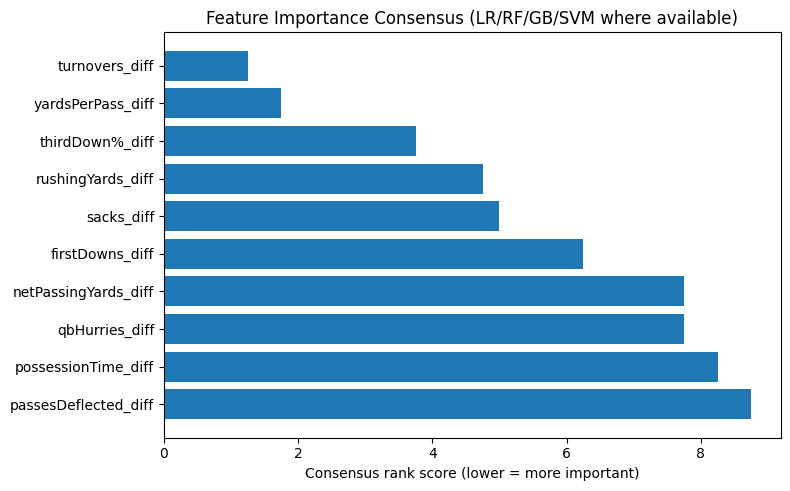
\includegraphics[width=0.9\textwidth]{feature_importance_consensus.png}
\caption{Consensus feature importance across fitted models (lower rank score indicates greater importance).}
\label{fig:feature_importance_consensus}
\end{figure}
\FloatBarrier

The consensus ranking places \textit{turnovers\_diff}, \textit{yardsPerPass\_diff}, \textit{thirdDown\%\_diff}, \textit{rushingYards\_diff}, and \textit{sacks\_diff} among the most influential predictors. This aligns with the EDA findings that turnover margin, efficiency, and pressure metrics are central drivers in one-score outcomes.

\section{Examining the College Football Playoff}
The College Football Playoff National Championship was played on January 19th, 2026 in the Hard Rock Stadium in Miami, FL. Featuring top-seed favorite Indiana University and 10-seed underdog University of Miami. Indiana's 27 - 21 victory over the Miami Hurricanes marked the end of the playoffs. Including the championship game, four out of the eleven games played in the tournament ended in a one-score point differential, and can be analyzed by our models. The other three matchups were Texas A and M vs. University of Miami (3 - 10), University of Georgia vs. Ole Miss (34 - 39), and Ole Miss vs. University of Miami (27 - 31). Firstly, in three of these matchups (all except the championship game), the lower seeded team managed to win, further showing the unpredictable nature of these one-score matchups.

For each of these four games, we constructed the same twelve difference features used in training (home minus away, aligned with the home/away designation in the underlying game record). Table \ref{tab:cfp_one_score_predictions} lists predicted winners with games as columns and models as rows; the last column counts how many of the four games each model classified correctly, and the bottom row counts how many of the five models matched the actual winner in each game. Predicted winners are obtained by mapping model output to team names: class $1$ indicates a predicted win for the designated home team and class $0$ a predicted win for the designated away team.\footnote{For example, in the Georgia vs. Ole Miss statistics used here, Georgia is the designated home team; all models output class $0$, i.e., a predicted win for Ole Miss.} On this small postseason sample, all models reach consensus on the games' results. Two matchups (Georgia vs. Ole Miss and Ole Miss vs. Miami) are classified correctly by all five models, and two (Texas A\&M vs. Miami and the championship game) by none.

\begin{table}[H]
\centering
\footnotesize
\setlength{\tabcolsep}{3pt}
\begin{tabular}{@{}lcccc c@{}}
\toprule
\textbf{Model} & \shortstack{\textbf{TAMU--MIA}\\(3--10)} & \shortstack{\textbf{UGA--OM}\\(34--39)} & \shortstack{\textbf{OM--MIA}\\(27--31)} & \shortstack{\textbf{IND--MIA}\\(27--21)} & \textbf{\shortstack{Games\\correct}} \\
\midrule
\textbf{Actual winner} & Miami & Ole Miss & Miami & Indiana & --- \\
\midrule
Logistic regression & Texas A\&M & Ole Miss & Miami & Miami & 2/4 \\
Random forest & Texas A\&M & Ole Miss & Miami & Miami & 2/4 \\
Gradient boosting & Texas A\&M & Ole Miss & Miami & Miami & 2/4 \\
SVM & Texas A\&M & Ole Miss & Miami & Miami & 2/4 \\
Naive Bayes & Texas A\&M & Ole Miss & Miami & Miami & 2/4 \\
\midrule
\textbf{Models correct (of 5)} & 0/5 & 5/5 & 5/5 & 0/5 & --- \\
\bottomrule
\end{tabular}
\caption{2025 College Football Playoff one-score games: each column is a game (score in parentheses); each row is a fitted model's predicted winner. The \emph{Games correct} column is the number of games whose winner that model predicted correctly (out of four). The bottom row is the number of models whose prediction matched the actual winner for that game (out of five).}
\label{tab:cfp_one_score_predictions}
\end{table}
\FloatBarrier

The predictions were generated in \texttt{Predictions.py} by passing each feature row through every trained estimator imported from \texttt{MachineLearning.py}; see the following excerpt.

\begin{lstlisting}
FEATURE_NAMES = [  # same 12 columns as final_data_EDA.csv
    "possessionTime_diff", "turnovers_diff", "yardsPerRushAttempt_diff",
    "rushingYards_diff", "yardsPerPass_diff", "netPassingYards_diff",
    "firstDowns_diff", "tacklesForLoss_diff", "sacks_diff",
    "qbHurries_diff", "passesDeflected_diff", "thirdDown%_diff",
]
GAMES = [
    ("Texas A&M @ Miami (TexMia)", TexMia),
    ("Georgia @ Ole Miss (GeoOM)", GeoOM),
    # ... remaining matchups ...
]
MODELS = [
    ("Logistic Regression", log_reg),
    ("Random Forest", rf_model),
    # ... other estimators ...
]

for game_label, game in GAMES:
    X = pd.DataFrame([game], columns=FEATURE_NAMES)
    for model_name, model in MODELS:
        pred = int(model.predict(X)[0])
        proba = model.predict_proba(X)[0]
\end{lstlisting}


\section{Limitations}
Even with a very a small sample, this examination of the College Football Playoff clearly illustrates some of the limitations with our fitted models. Firstly, they were trained on the conditional task of same-game statistics within historical one-score FBS games. Thus, our models cannot be used as forecasters of future matchups. Secondly, football at all levels includes luck, randomness, and essentially infinite hard-to-track variables that are difficult to capture with box-score features alone. This is simply the nature of sports analytics. Even models trained on millions of data points will struggle to reach high accuracy, especially for close matchups. However, it is important to note that the unpredictability of sports is what keeps billions of fans across the world engaged with their favorite sports leagues, teams, and players. Our successful, yet limited, models show, not only the capabilities of machine learning in the vast field of sports, but also the exact unpredictability that shapes the sports we love.

% \section{Game Forecasting}
% Using the five trained classification models, predictions were generated for the 2025 College Football Playoff matchups in the form of bracket outcomes. These predictions were constructed by computing each team's average difference statistics from regular season games throughout the 2025 season, and then forming matchup-specific feature vectors by subtracting the away team’s averages from those of the home team. The resulting feature vectors were passed into the trained models to obtain predicted probabilities of a home-team victory, which were subsequently used to determine bracket advancement.

% It is important to note that all models used for these predictions were trained exclusively on games that concluded with a one-score margin. As a result, the learned relationships between feature differentials and game outcomes are conditioned on competitive game states in which the final margin of victory was small. Consequently, the predictions presented here should be interpreted as estimates of relative team strength under the assumption of a close contest, rather than unconditional forecasts of game outcomes.

% Since there was no guarantee that these postseason games would end in one-score margins, the applicability of these predictions is inherently quite limited. Games that result in large margins of victory may exhibit different statistical dynamics than those captured by the training data, and therefore may not be well represented by the model. This limitation reflects a deliberate modeling choice rather than a methodological flaw, as this thesis is explicitly focused on understanding outcome determinants in closely contested games.

% Under this framework, bracket predictions should be viewed as counterfactual outcomes: namely, which team would be expected to prevail if the matchup were to end within a one-score difference. This perspective aligns with the study’s objective of isolating performance factors that differentiate teams in high-leverage, evenly matched situations, such as late-game execution, efficiency, and turnover margins. Our five models produced the following brackets:
% \FloatBarrier
% \begin{figure}
%     \centering
%     \includegraphics[width=\textwidth]{Bracket - Logistic Regression.png}\par\vspace{6pt}
%     \caption{Tournament bracket created by our Logistic Regression model - Indiana Predicted Winner}
% \end{figure}
% \begin{figure}
%     \includegraphics[width=\textwidth]{Bracket - Naive Bayes.png}\par\vspace{6pt}
%     \caption{Tournament bracket created by our Naive Bayes model - Indiana Predicted Winner}
% \end{figure}
% \begin{figure}
%     \centering
%     \includegraphics[width=\textwidth]{Bracket - Random Forest.png}\par\vspace{6pt}
%     \caption{Tournament bracket created by our Random Forest model - Indiana Predicted Winner}
% \end{figure}
% \begin{figure}
%     \includegraphics[width=\textwidth]{Bracket - Gradient Boosting.png}\par\vspace{6pt}
%     \caption{Tournament bracket created by our Gradient Boost model - Indiana Predicted Winner}
% \end{figure}
% \begin{figure}
%     \includegraphics[width=\textwidth]{Bracket - SVM.png}
%     \caption{Tournament bracket created by our Support Vector Machine model - James Madison Predicted Winner}
% \end{figure}
% \FloatBarrier
% Observing the brackets above, we see that all models, except for the Support Vector Machine, predict Indiana University (ranked 1st in the AP Poll and 2nd betting favorite across multiple sportsbooks) to win the championship. Although most models agreed on the overall winner, the models differ substantially in the predicted outcomes of individual matchups throughout the first round, quarterfinals, and semifinals. The College Football Playoff National Championship was played on January 19th, 2026 in the Hard Rock Stadium in Miami, FL. Featuring top-seed favorite Indiana University and 10-seed underdog University of Miami. Indiana's 27 - 21 victory over the Miami Hurricanes marked the end of the playoffs, resulting in the following tournament bracket:
% \FloatBarrier
% \begin{figure}
%     \includegraphics[width=\textwidth]{Final Bracket.png}
%     \caption{Official 2025 College Football Playoff Bracket}
% \end{figure}
% \FloatBarrier
% After comparing the true results to our models' predictions, we observe that four out of the five models correctly predicted Indiana University to finish as champions. Even more impressive, however, was the Naive Bayes model correctly predicting 10-seed University of Miami to upset 2-seed Ohio State University. This prediction, although the game did not end in a one-score difference, was correct despite the majority of fans and analysts predicting Ohio State to easily defeat Miami in this quarterfinals matchup. Although it is important to keep in mind the limitations of using our ``one-score game'' models to predict future matchups, they did perform surprisingly well:
% \FloatBarrier
% \begin{figure}
%     \includegraphics[width=\textwidth]{Bracket Scores.png}
%     \caption{Accuracy scores for predictions via each model. Naive Bayes performed quite well with a ~73\% accuracy, and SVM performed extremely poorly with an accuracy of ~18\%}
% \end{figure}
% \FloatBarrier

\appendix
% Uniform width for appendix-only plots (keeps the appendix shorter).
\newcommand{\AppFigW}{0.48\textwidth}

\section{Explanation of Statistical Features}
\label{app:stat_features}

\begin{itemize}
    \item \textbf{possessionTime}: Amount of game time (in seconds) that a team had possession of the football.
    \item \textbf{interceptions}: Amount of times a team on offense (unintentionally) threw the ball to a defensive player.
    \item \textbf{fumblesLost}: Amount of times a team on offense (unintentionally) dropped the ball from their possession during a live play for it to be picked up by a defensive player.
    \item \textbf{turnovers}: Amount of times a team on offense (unintentionally) lost possession of the football (typically fumbles and interceptions).
    \item \textbf{yardsPerRushAttempt}: Amount of yards gained per rushing attempt by a team's offense.
    \item \textbf{rushingYards}: Total amount of yards gained by a team's rushing offense.
    \item \textbf{yardsPerPass}: Amount of yards gained per passing attempt by a team's offense.
    \item \textbf{netPassingYards}: Total amount of yards gained by a team's passing offense.
    \item \textbf{totalYards}: Total amount of yards gained by a team's offense.
    \item \textbf{firstDowns}: Amount of times a team progressed ten yards, gaining themselves a new set of four downs.
    \item \textbf{tacklesForLoss}: Amount of times a team's defense tackled an offensive player with the ball behind the line of scrimmage.
    \item \textbf{tackles}: Amount of times a team's defense tackled an offensive player with the ball.
    \item \textbf{sacks}: Amount of times a team's defense tackled the offense's quarterback while he held possession and made no attempt to run for forward yardage.
    \item \textbf{qbHurries}: Amount of times a team's defensive efforts forced the offense's quarterback to throw the ball earlier than intended, scramble, or alter his throw (that did not result in a sack).
    \item \textbf{passesDeflected}: Amount of times a team's defense blocked the offense's throw leading to no catch being made.
    \item \textbf{thirdDown\%}: The percentage of third down plays a team successfully converted into a first down.
\end{itemize}
\FloatBarrier

\section{ROC curves (2025 holdout)}
\label{app:roc}

Each plot shows the receiver operating characteristic (ROC) curve for one fitted classifier evaluated on the held-out 2025 one-score test set, with the dashed diagonal corresponding to random guessing. Curves were generated in \texttt{MachineLearning.py} using predicted class probabilities (or decision-function scaled scores where needed) against true labels \cite{fawcett2006introduction}.

\begin{figure}[H]
\centering

\includegraphics[width=\AppFigW]{\detokenize{Figures/ROC Curves/ROC_Logistic Regression.png}}
\caption{ROC curve: logistic regression.}
\label{appfig:roc_lr}
\end{figure}

\begin{figure}[H]
\centering

\includegraphics[width=\AppFigW]{\detokenize{Figures/ROC Curves/ROC_Random Forest.png}}
\caption{ROC curve: random forest.}
\label{appfig:roc_rf}
\end{figure}

\begin{figure}[H]
\centering

\includegraphics[width=\AppFigW]{\detokenize{Figures/ROC Curves/ROC_Gradient Boosting.png}}
\caption{ROC curve: gradient boosting.}
\label{appfig:roc_gb}
\end{figure}

\begin{figure}[H]
\centering

\includegraphics[width=\AppFigW]{\detokenize{Figures/ROC Curves/ROC_SVM.png}}
\caption{ROC curve: support vector machine (probability enabled).}
\label{appfig:roc_svm}
\end{figure}

\begin{figure}[H]
\centering

\includegraphics[width=\AppFigW]{\detokenize{Figures/ROC Curves/ROC_Naive Bayes.png}}
\caption{ROC curve: Gaussian naive Bayes.}
\label{appfig:roc_nb}
\end{figure}
\FloatBarrier

\section{Confusion matrices (2025 holdout)}
\label{app:cm}

Each heatmap summarizes predictions on the held-out 2025 one-score test set: rows correspond to the true label (class~$0$: away-team win; class~$1$: home-team win) and columns to the model's predicted label, matching \texttt{scikit-learn}'s default convention for binary confusion matrices \cite{pedregosa2011scikit}. Diagonal entries are correct classifications; off-diagonal entries are errors. Figures were produced in \texttt{MachineLearning.py}.

\begin{figure}[H]
\centering

\includegraphics[width=\AppFigW]{\detokenize{Figures/Confusion Matrices/CM_Logistic Regression.png}}
\caption{Confusion matrix: logistic regression (2025 test).}
\label{appfig:cm_lr}
\end{figure}

\begin{figure}[H]
\centering

\includegraphics[width=\AppFigW]{\detokenize{Figures/Confusion Matrices/CM_Random Forest.png}}
\caption{Confusion matrix: random forest (2025 test).}
\label{appfig:cm_rf}
\end{figure}

\begin{figure}[H]
\centering

\includegraphics[width=\AppFigW]{\detokenize{Figures/Confusion Matrices/CM_Gradient Boosting.png}}
\caption{Confusion matrix: gradient boosting (2025 test).}
\label{appfig:cm_gb}
\end{figure}

\begin{figure}[H]
\centering

\includegraphics[width=\AppFigW]{\detokenize{Figures/Confusion Matrices/CM_SVM.png}}
\caption{Confusion matrix: support vector machine (2025 test).}
\label{appfig:cm_svm}
\end{figure}

\begin{figure}[H]
\centering

\includegraphics[width=\AppFigW]{\detokenize{Figures/Confusion Matrices/CM_Naive Bayes.png}}
\caption{Confusion matrix: Gaussian naive Bayes (2025 test).}
\label{appfig:cm_nb}
\end{figure}
\FloatBarrier

\section{Feature importance plots}
\label{app:feature-importance}

These bar plots mirror the feature-importance summaries saved from \texttt{MachineLearning.py}: absolute standardized coefficients for linear models (logistic regression and linear-kernel SVM) and mean decrease in impurity for tree ensembles. The consensus aggregation is only shown in the main text (Figure~\ref{fig:feature_importance_consensus}); Gaussian naive Bayes does not produce a comparable global importance vector in this pipeline.

\begin{figure}[H]
\centering

\includegraphics[width=\AppFigW]{\detokenize{Figures/Feature Importance/feature_importance_lr.png}}
\caption{Feature importance: logistic regression (absolute coefficients on the standardized scale).}
\label{appfig:fi_lr}
\end{figure}

\begin{figure}[H]
\centering

\includegraphics[width=\AppFigW]{\detokenize{Figures/Feature Importance/feature_importance_rf.png}}
\caption{Feature importance: random forest.}
\label{appfig:fi_rf}
\end{figure}

\begin{figure}[H]
\centering

\includegraphics[width=\AppFigW]{\detokenize{Figures/Feature Importance/feature_importance_gb.png}}
\caption{Feature importance: gradient boosting.}
\label{appfig:fi_gb}
\end{figure}

\begin{figure}[H]
\centering

\includegraphics[width=\AppFigW]{\detokenize{Figures/Feature Importance/feature_importance_svm_linear.png}}
\caption{Feature importance: linear SVM (magnitude of coefficients).}
\label{appfig:fi_svm}
\end{figure}
\FloatBarrier

\newpage
\printbibliography


\end{document}